\documentclass[12pt,a4paper,leqno]{report}

\usepackage[UTF8]{inputenc}
\usepackage[T1]{fontenc}
\usepackage[finnish]{babel}
\usepackage{amsthm}
\usepackage{amsfonts}         
\usepackage{amsmath}
\usepackage{amssymb}
\usepackage{graphicx}

\pagestyle{plain}
\setcounter{page}{1}
\addtolength{\hoffset}{-1.15cm}
\addtolength{\textwidth}{2.3cm}
\addtolength{\voffset}{0.45cm}
\addtolength{\textheight}{-0.9cm}

\title{Tietokantasovellus: Keskustelufoorumi (dokumentaatio)}
\author{Wille Lehtomäki}
\date{}

\begin{document}

\maketitle

\tableofcontents

\chapter{Johdanto}\label{johd}

Työssä toteutetaan PHP-kielellä keskustelufoorumi, jonka käyttämiseen (siis pelkkään lukemiseenkin) tarvitaan käyttäjätunnus. Foorumilla on yksi ylläpitäjä, joka voi tavallisen käyttäjän oikeuksien lisäksi myös esimerkiksi poistaa viestejä ja lisätä viesteille aihekategorioita.

Foorumi käyttää PostgreSQL-tietokantaa.

\chapter{Yleiskuva järjestelmästä}

\begin{center}
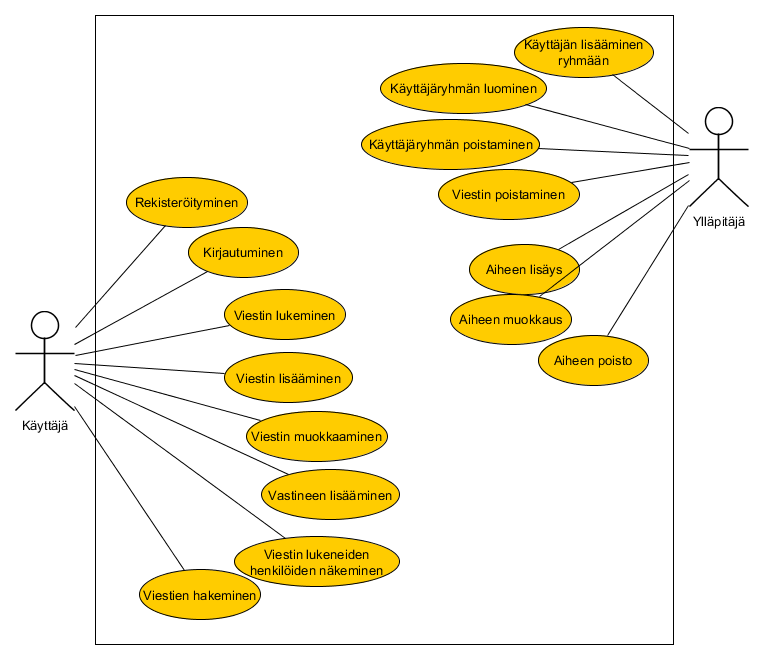
\includegraphics[scale=0.5]{kayttp}
\end{center}

\noindent \textbf{Huom:} Ylläpitäjä voi tehdä kaikki samat asiat kuin Käyttäjäkin, mutta luettavuuden vuoksi nämä yhteydet on jätetty kaaviossa merkitsemättä.

\Large\textbf{Käyttäjäryhmät}\normalsize\\

\emph{Käyttäjä} on foorumin ns. "tavallinen"  käyttäjä, eli henkilö, joka voi esimerkiksi lukea ja kirjoittaa viestejä.\\

Foorumin \emph{ylläpitäjällä} on lisäksi oikeus mm. poistaa viestejä ja määritellä viesteille aihealueita niiden järjestelemiseksi sekä hallita käyttäjäryhmiä.\\ \\

\Large\textbf{Käyttötapauskuvauksia}\normalsize\\

\textbf{Viestin lisääminen}

\noindent Käyttäjä kirjoittaa ja lisää foorumille uuden aloitusviestin, eli viestin, joka ei ole vastine mihinkään vanhaan viestiin. Muut käyttäjät voivat sekä lukea viestin että kirjoittaa sille vastineita.\\

\textbf{Vastineen lisääminen}

\noindent Vastine on vastausviesti johonkin aiemmin kirjoitettuun viestiin.\\

\textbf{Viestin lukeneiden näkeminen}

\noindent Käyttäjälle näytetään lista kaikista käyttäjistä, jotka ovat lukeneet tietyn viestin.\\

\textbf{Viestien hakeminen}

\noindent Viestejä voi hakea kirjoittajan, aiheen tai kirjoituspäivän perusteella.\\

\textbf{Viestin poistaminen}

\noindent Ylläpitäjä voi poistaa joko yksittäisiä vastineita tai kokonaisen viestiketjun poistamalla ketjun aloitusviestin.\\

\textbf{Käyttäjäryhmän luominen}

\noindent Ylläpitäjä voi luoda käyttäjille ryhmiä.\\

\textbf{Aiheen lisäys}

\noindent Käyttäjien ryhmittelyn lisäksi ylläpitäjä voi ryhmitellä myös viestejä asettamalla viesteille eri aihealueita, joihin kukin viesti mahdollisine vastineineen kuuluu.\\

\noindent Loput käyttötapaukset on listattu käyttötapauskaaviossa.

\end{document}